\section{Digital to Analog Converter}
\subsection{Prediction}
% TODO: Prediction graph

\subsection{Discrete DAC}
The provided DAC schematic was captured in Cadence PSpice as shown in
Figure~\ref{f:dac_schem}.
%
\begin{figure}[H]
\centering
	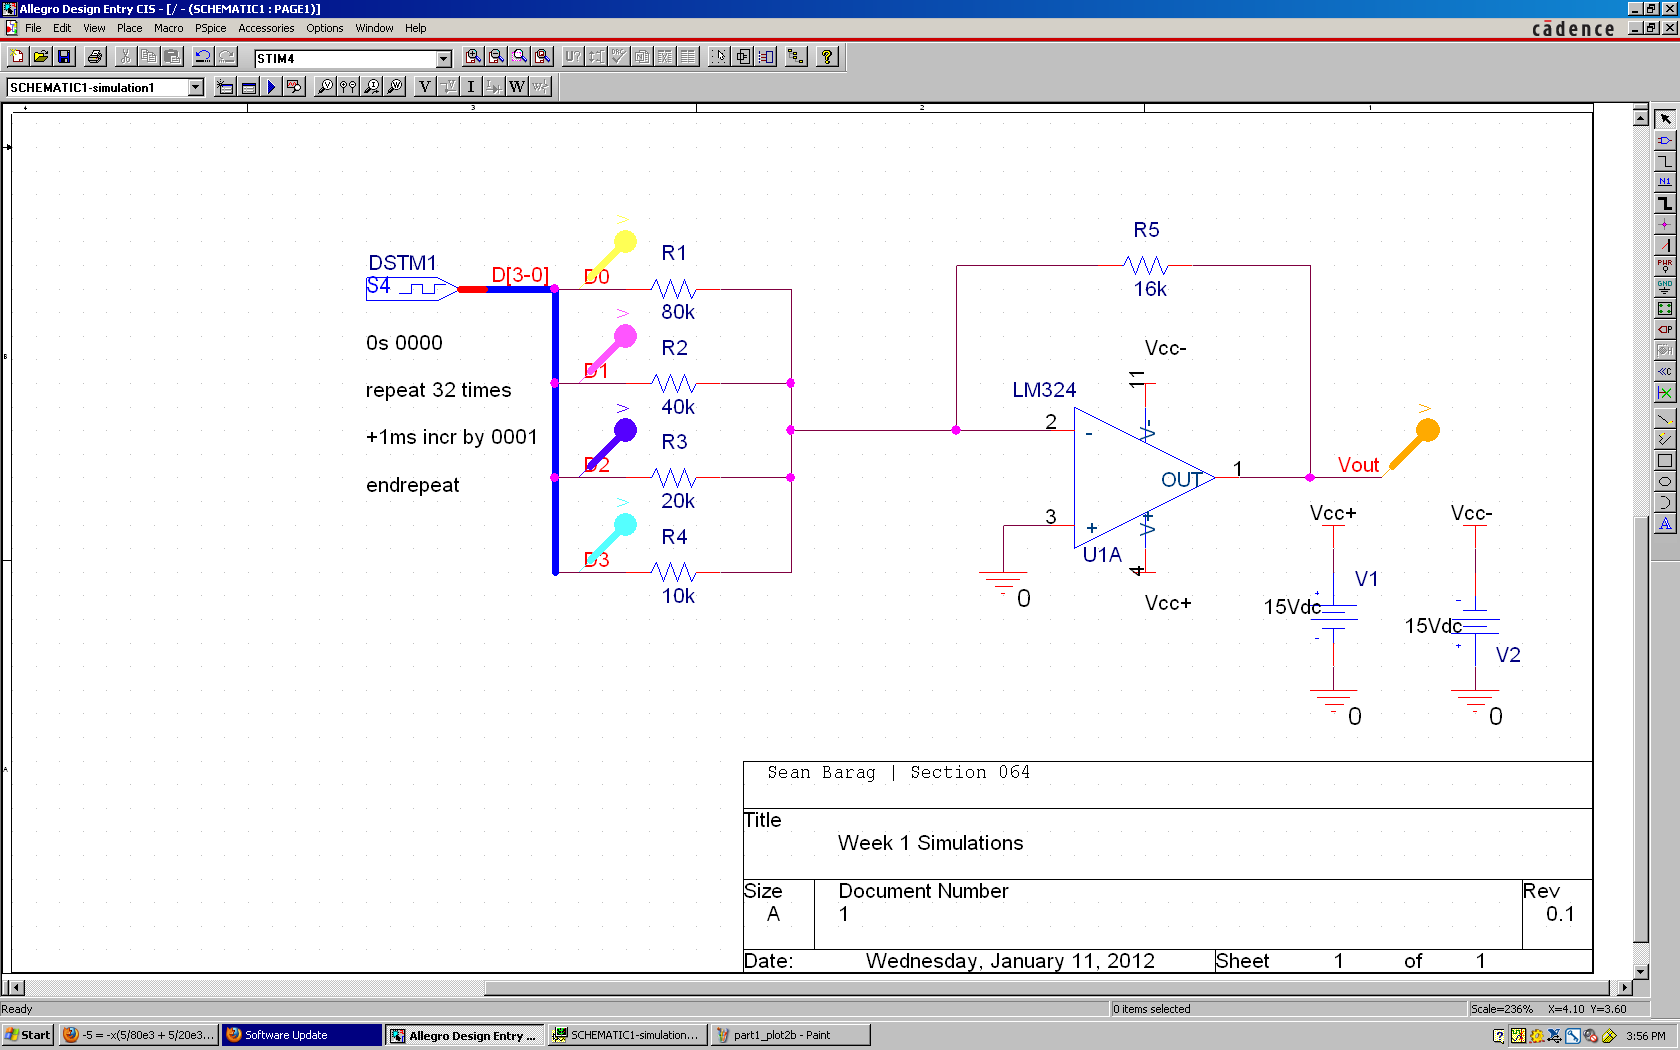
\includegraphics[width=.8\textwidth]{img/shot/part1_schem.PNG}
	\parbox{.8\textwidth}{
	\caption[Discrete DAC --- Schematic]{Provided schematic for the discrete digital to analog converter (DAC).  Note that the value of~$R_5$ has already been adjusted in this image.}
	\label{f:dac_schem}}
\end{figure}
%
Note that the element titled ``DTSM 1'' was edited to repeatedly count from
zero~($0000_2$) to fifteen~($1111_2$) with each intermediate value
lasting for~\SI{1}{\milli\second}.  This was accomplished by editing the element properties and providing the four instructions shown:
%
\begin{itemize*}
	\item \ttt{0s 0000}
	\item \ttt{repeat 32 times}
	\item \ttt{+1ms incr by 00001}
	\item \ttt{endrepeat}
\end{itemize*}
%
This circuit was simulated using transient analysis for the
required~\SI{32}{\milli\second}, allowing one full input count-up cycle to be
observed.  The voltage at each bit, along with the output voltage, is plotted
below in Figure~\ref{f:dac_plot1}.
%
\begin{figure}[H]
\centering
	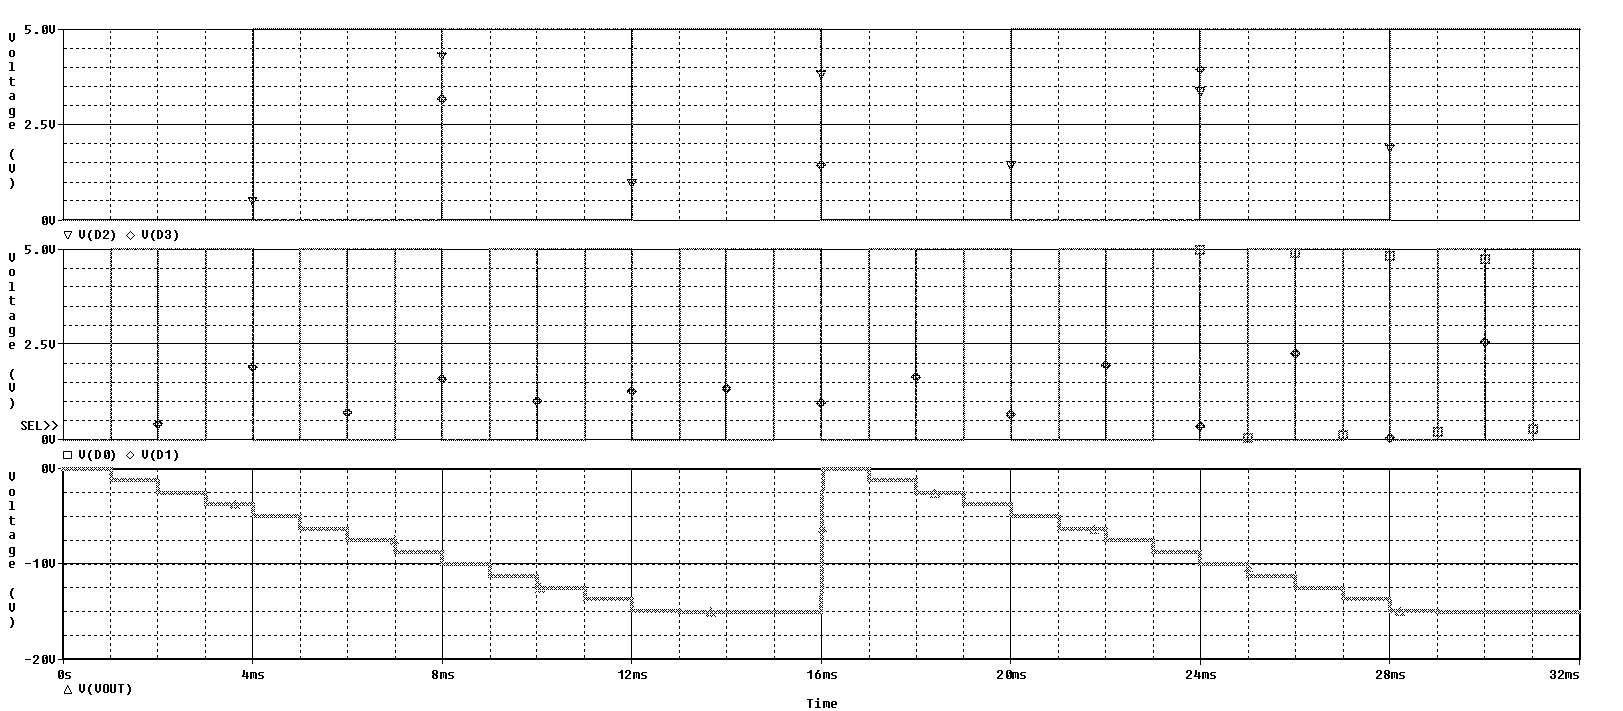
\includegraphics[width=.8\textwidth]{img/plot/part1_plot1b.PNG}
	\parbox{.8\textwidth}{
	\caption[Discrete DAC --- Initial Results]{Initial simulation results for
	the discrete DAC.  Note that the output reaches a lower threshold as a
	result of the value of~$R_5$.}
	\label{f:dac_plot1}}
\end{figure}
%
As is shown in the produced plot of output voltage versus time, the output
reaches the minimum possible output voltage of~\SI{-15}{\volt} at~\SI{12}{\milli\second}.  This is
caused by an improperly tuned feedback resistor~$R_5$.

\subsection{Feedback Resistor Tuning}
In order to ensure that the minimum output voltage of~\SI{-15}{\volt}~(limited
by the op amp's supply voltage) occurs at the maximum input value of~$1111_2$,
the value of the feedback resistor~$R_5$ must be adjusted.  The output voltage of the discrete DAC is governed by~\eqref{eq:dac}:
%
\begin{equation}
	V_\text{out} = - 5 R_5 \left( \frac{D_3}{R_4} + \frac{D_2}{R_3} + \frac{D_1}{R_2} + \frac{D_0}{R_1} \right)
	\label{eq:dac}
\end{equation}
%
where~$D_0$ through~$D_3$ are the binary values of the corresponding bits in
Figure~\ref{f:dac_schem} and~$R_1$ through~$R_5$ are the associated resistors
in the same schematic.  By designing for a binary value of~0101 to correspond
with a~\SI{-5}{\volt} output, we can ensure that the full-scale output will
fall at~\SI{-15}{\volt}.
%
\begin{align*}
	V_\text{out} = \SI{-5}{\volt} &= -5 R_5 \left( \frac{0}{\SI{10}{\kilo\ohm}} + \frac{1}{\SI{20}{\kilo\ohm}} + \frac{0}{\SI{40}{\kilo\ohm}} + \frac{1}{\SI{80}{\kilo\ohm}} \right) \\
	R_5 &= \frac{ -5 } { -5 \left( \frac{1}{\SI{20}{\kilo\ohm}} + \frac{1}{\SI{80}{\kilo\ohm}} \right) } \\
	    &= \SI{16}{\kilo\ohm}
\end{align*}
%
After completing these calculations, an appropriate value of~$R_5$ was
determined to be~\SI{16}{\volt}.

\subsection{Adjusted Simulation}
The value of~$R_5$ was changed in the schematic and the simulation was run
again with the same~\SI{32}{\milli\second} duration.  Upon the simulation's
completion, PSpice produced the plot shown in Figure~\ref{f:dac_plot2}, below.
%
\begin{figure}[H]
\centering
	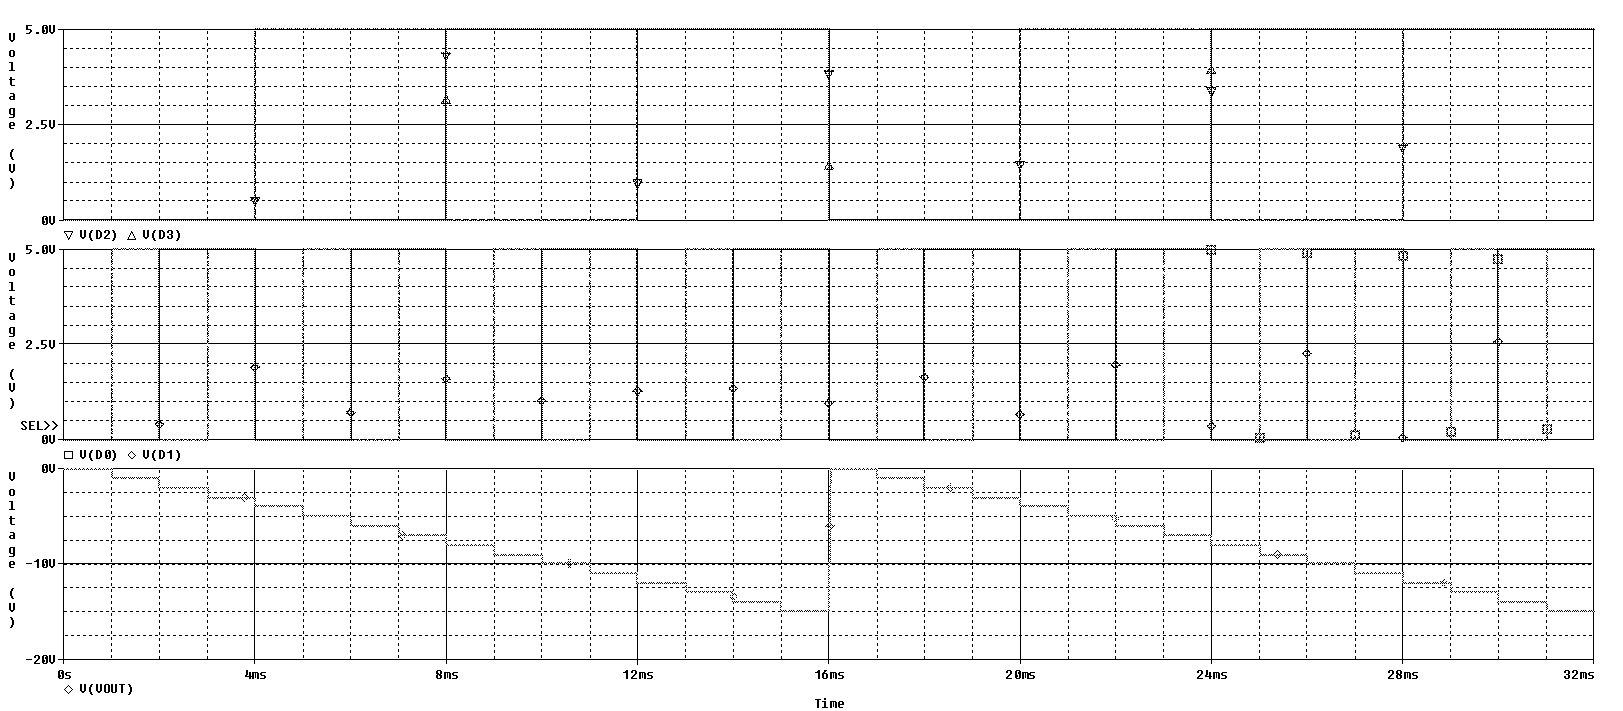
\includegraphics[width=.8\textwidth]{img/plot/part1_plot2b.PNG}
	\parbox{.8\textwidth}{
	\caption[Discrete DAC --- Tuned Results]{Final simulation results with an adjusted feedback resistor.}
	\label{f:dac_plot2}}
\end{figure}

\subsection{Discrete DAC Results}
As is shown in the above include PSpice plot, the digital to analog converter produces an accurate representation of the input bits.  By adjusting the
